\documentclass[12pt, a4paper]{article}

\usepackage{lastpage}
\usepackage{mathtools}
\usepackage{xltxtra}
\usepackage{libertine}
\usepackage{amsmath}
\usepackage{amsthm}
\usepackage{amsfonts}
\usepackage{amssymb}
\usepackage{enumitem}
\usepackage{xcolor}
\usepackage[left=1.5cm, right=1.5cm, top=2cm, bottom=2cm, bindingoffset=0cm, headheight=15pt]{geometry}
\usepackage{fancyhdr}
\usepackage[russian]{babel}
% \usepackage[utf8]{inputenc}
\usepackage{catchfilebetweentags}
\usepackage{accents}
\usepackage{calc}
\usepackage{etoolbox}
\usepackage{mathrsfs}
\usepackage{wrapfig}

\providetoggle{useproofs}
\settoggle{useproofs}{false}

\pagestyle{fancy}
\lfoot{M3137y2019}
\rhead{\thepage\ из \pageref{LastPage}}

\newcommand{\R}{\mathbb{R}}
\newcommand{\Q}{\mathbb{Q}}
\newcommand{\C}{\mathbb{C}}
\newcommand{\Z}{\mathbb{Z}}
\newcommand{\B}{\mathbb{B}}
\newcommand{\N}{\mathbb{N}}

\newcommand{\const}{\text{const}}

\newcommand{\teormin}{\textcolor{red}{!}\ }

\DeclareMathOperator*{\xor}{\oplus}
\DeclareMathOperator*{\equ}{\sim}
\DeclareMathOperator{\Ln}{\text{Ln}}
\DeclareMathOperator{\sign}{\text{sign}}
\DeclareMathOperator{\Sym}{\text{Sym}}
\DeclareMathOperator{\Asym}{\text{Asym}}
% \DeclareMathOperator{\sh}{\text{sh}}
% \DeclareMathOperator{\tg}{\text{tg}}
% \DeclareMathOperator{\arctg}{\text{arctg}}
% \DeclareMathOperator{\ch}{\text{ch}}

\DeclarePairedDelimiter{\ceil}{\lceil}{\rceil}
\DeclarePairedDelimiter{\abs}{\left\lvert}{\right\rvert}

\setmainfont{Linux Libertine}

\theoremstyle{plain}
\newtheorem{axiom}{Аксиома}
\newtheorem{lemma}{Лемма}

\theoremstyle{remark}
\newtheorem*{remark}{Примечание}
\newtheorem*{exercise}{Упражнение}
\newtheorem*{consequence}{Следствие}
\newtheorem*{example}{Пример}
\newtheorem*{observation}{Наблюдение}

\theoremstyle{definition}
\newtheorem{theorem}{Теорема}
\newtheorem*{definition}{Определение}
\newtheorem*{obozn}{Обозначение}

\setlength{\parindent}{0pt}

\newcommand{\dbltilde}[1]{\accentset{\approx}{#1}}
\newcommand{\intt}{\int\!}

% magical thing that fixes paragraphs
\makeatletter
\patchcmd{\CatchFBT@Fin@l}{\endlinechar\m@ne}{}
  {}{\typeout{Unsuccessful patch!}}
\makeatother

\newcommand{\get}[2]{
    \ExecuteMetaData[#1]{#2}
}

\newcommand{\getproof}[2]{
    \iftoggle{useproofs}{\ExecuteMetaData[#1]{#2proof}}{}
}

\newcommand{\getwithproof}[2]{
    \get{#1}{#2}
    \getproof{#1}{#2}
}

\newcommand{\import}[3]{
    \subsection{#1}
    \getwithproof{#2}{#3}
}

\newcommand{\given}[1]{
    Дано выше. (\ref{#1}, стр. \pageref{#1})
}

\renewcommand{\ker}{\text{Ker }}
\newcommand{\im}{\text{Im }}
\newcommand{\grad}{\text{grad}}

\lhead{Дискретная математика}
\cfoot{}
\rfoot{Лекция 7}

\usepackage{listings}
\usepackage{courier}
\lstset{basicstyle=\footnotesize\ttfamily,breaklines=true}
\lstset{framextopmargin=50pt,frame=bottomline}

\begin{document}

\begin{definition}
    Конечное, непустое множество $\Sigma$ --- \textbf{алфавит}
\end{definition}

\begin{example}
    \begin{itemize}
        \item $\{0, 1\}$
        \item $\{a, b, c\ldots z\}$
        \item Unicode
    \end{itemize}
\end{example}

$$\Sigma^*:=\bigcup_{k=0}^\infty \Sigma^k$$

\begin{definition}
    \textbf{Конкатенация}:
    $$\Sigma^k\times \Sigma^l \to \Sigma^{k+l}$$
    Это аддитивная операция с нейтральным элементом.
\end{definition}

\begin{definition}
    \textbf{Язык} над алфавитом $\Sigma^*$ --- подмножество $\Sigma^*$
\end{definition}

$\Sigma^*$ --- бесконечное счётное множество

Множество всех языков $2^{\Sigma^*}$, т.к. каждый из элементов $\Sigma^*$ либо включен, либо нет. Это множество несчетно.

\begin{example}
    \begin{enumerate}
        \item $A=\{w | \text{ в } w \text{ четное число нулей}\}\subset \{0, 1\}^*$
        
        $01011\in A \quad 000\not\in A$
        \item $Pal=\{w | w \text{ --- палиндром}\}\subset \{0, 1\}^*$
        
        $010\in Pal \quad 0000\in Pal \quad 01\not\in Pal$
    \end{enumerate}
\end{example}

Языки надо задавать формально, а не что-то рода \textit{``язык палиндромов''}. Есть два способа это делать:
\begin{enumerate}
    \item \textbf{Распознавание}: есть черный ящик, который на вход получает слово и выдает булево значение --- принадлежит слово искомому языку или нет.
    \item \textbf{Конструирование}: система правил диктует то, как устроены слова в искомом языке.
\end{enumerate}

\begin{example}
    Распознавание ПСП:

    Тут код.
\end{example}

\begin{example}
    Конструирование ПСП:

    $\varepsilon$ --- ПСП
    
    $A$ --- ПСП $\Rightarrow (A)$ --- ПСП

    $A, B$ --- ПСП $\Rightarrow AB$ --- ПСП
\end{example}

Автоматы распознают принадлежность слова языку.
\begin{definition}
    \textbf{Детерменированный конечный автомат \textit{(ДКА)}}:
    \begin{enumerate}
        \item Состояния, обозначаемые кругами
        \item Переходы, обозначаемые ребрами между состояниями и помечаемые символом алфавита. Из любого состояния есть ровно один переход по каждому символу алфавита.
        \item Начальное состояние, обозначаемое входящей стрелкой из никуда
        \item Допускающие состояния, обозначаемые кругом внутри себя.
    \end{enumerate}
\end{definition}

\begin{figure}
    \centering
    \begin{minipage}{.5\textwidth}
      \centering
      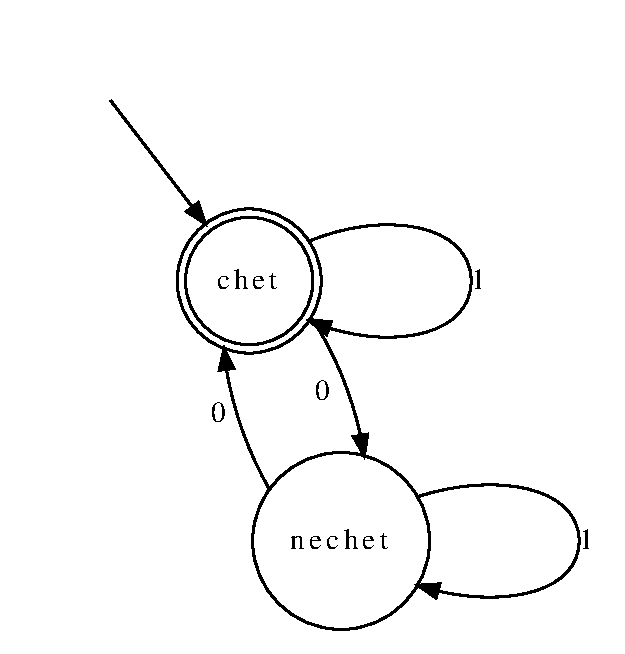
\includegraphics[scale=0.7]{graphs/A.eps}
      \caption{Автомат для $\{w | \text{ в } w \text{ четное число нулей}\}$}
    %   \label{fig:test1}
    \end{minipage}%
    \begin{minipage}{.5\textwidth}
      \centering
      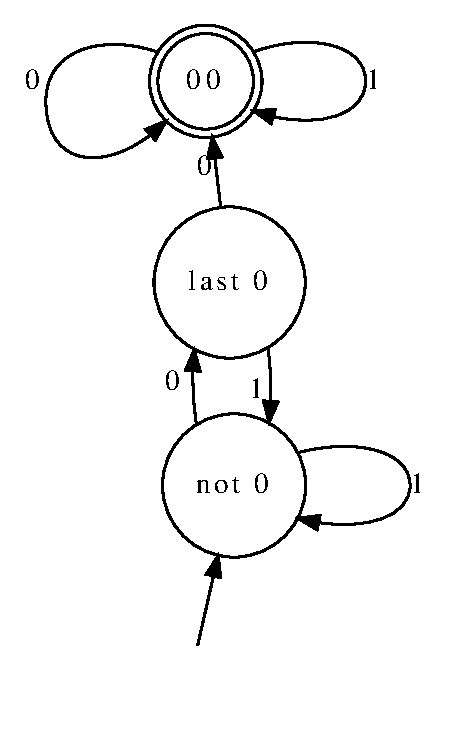
\includegraphics[scale=0.7]{graphs/ZZ.eps}
      \caption{Автомат $\{w | \text{ в } w \text{ содержит два нуля подряд}\}$}
    %   \label{fig:test2}
    \end{minipage}
\end{figure}

Переименуем состояния ``not $0$'' $\to$ $A$, ``last $0$'' $\to B$, ``$00$'' $\to C$.

Опишем математически ДКА:

\begin{definition}
    ДКА $AV=\langle \Sigma, Q, S\in Q, T\subset Q, \delta:Q\times\Sigma\to Q\rangle$

    \textbf{Мгновенное описание} $AV$ --- пара из состояния $A$ и оставшихся от исходного слова строки. Это объект из множества $Q\times \Sigma^*$, например $\langle A, 11011001\rangle$.

    На мгновенных описаниях можно задать отношение ``переходит за 1 шаг'', обозначим его $\vdash$. Формально оно задается следующим образом:

    $\langle p, \alpha\rangle\vdash \langle q, \beta\rangle$, если:
    \begin{enumerate}
        \item $\alpha=c\beta$
        \item $q=\delta(p, c)$
    \end{enumerate}

    Тогда для для слова $S$ верно следующее:
    $$\langle S, x\rangle\vdash \langle u_1, x_1\rangle\vdash\langle u_2, x_2\rangle\vdash\ldots\vdash \langle u_l, \varepsilon\rangle$$
    $$AV \text{ допускает } x \Leftrightarrow u_L\in T$$
    Эта запись неудобна, поэтому обозначим транзитивное замыкание $\vdash$ как $\vdash^*$, это --- отношение ``переходит $\geq 0$ шагов''. Тогда получается следующее:
    $$AV \text{ допускает } x \Leftrightarrow \langle s, x\rangle\vdash^*\langle t, \varepsilon\rangle$$
\end{definition}

Заметим, что все ДКА --- счётное множество, а языки - несчётное $\Rightarrow$ не любой язык можно описать с помощью ДКА. Назовем все языки, которые можно получить с помощью ДКА \textbf{автоматными}.

\begin{definition}
    \textbf{Базовые регулярные языки}:
    \begin{itemize}
        \item \O
        \item $\{\varepsilon\}$
        \item $\{c_i\} \quad \Sigma=\{c_1\ldots c_z\}$
    \end{itemize}
\end{definition}

Обозначим множество базовых регулярных языков над $\Sigma=\{0, 1\}$ как $R_0=\{\{\}, \{\varepsilon\}, \{0\}, \{1\}\}$

Зададим три операции над этими языками:
\begin{enumerate}
    \item Объединение: $A\cup B$
    \item Конкатенация: $\{ab\ |\ a\in A, b\in B\}$
    \item Замыкание Клини: $A^*=\bigcup\limits_{i=0}^\infty A^i$
\end{enumerate}

$$R_1:=\{M \ | \ M\in R_0 \text{ или } M=AB, A\in R_0, B\in R_0, M=A\cap B, A\in R_0, B\in R_0 \text{ или } M=A^*, A\in R_0\}$$
$$R_1=\{\{\}, \{\varepsilon\}, \{0\}, \{1\}, \{\varepsilon, 0\}, \{\varepsilon, 1\}, \{00\}, \{01\}, \{10\}, \{11\}, \{0\}^*, \{1\}^* \}$$

\begin{definition}
    \textbf{Регулярные языки}:
    $$Reg=\bigcup_{i=0}^\infty R_i$$
\end{definition}

\end{document}